%%=============================================================================
%% Ontwerp en implementatie van de testomgeving
%%=============================================================================

\chapter{Ontwerp en implementatie van de testomgeving}%
\label{ch:testomgeving}

Alvorens de converter te ontwikkelen, werd er eerst een manuele testomgeving opgezet die als referentie dient voor de gewenste uitvoer. Dit hoofdstuk beschrijft achtereenvolgens de keuzes van elke tool die aan de basis van deze omgeving ligt, de concrete implementatie met de bijhorende Ansible- en Vagrant-configuratiebestanden, alsook hoe deze is ontworpen aan de hand van een netwerk- en implementatiediagram (in PlantUML). De converter die in het volgende hoofdstuk (\nameref{ch:poc}) wordt ontwikkeld, moet voor deze diagrammen als invoer een functioneel equivalente omgeving als uitvoer produceren.

\section{Evaluatie en toolkeuze}%
\label{sec:toolkeuze}

De keuzes voor de tools (diagramformaat, \emph{configuration management}-tool, \emph{Infrastructure-as-Code}-tool en gastbesturingssysteem) die in deze testomgeving worden ingezet, werden onder andere bepaald op basis van de aanwezigheid binnen de opleiding \emph{Toegepaste Informatica} en de praktische haalbaarheid voor de context van de converter.

\subsection{Diagramformaat (PlantUML)}%

Zoals besproken in \nameref{sec:uml}, zijn \emph{Visual Paradigm} en \emph{draw.io} de voornaamste UML-tools binnen de opleiding, maar beide zijn GUI-gebaseerd en werken met een drag-en-drop systeem \autocite{Lu2023}, wat ze ongeschikt maakt als invoerformaat voor een converter. \emph{MermaidJS} is een tekstueel alternatief dat beter kan verwerkt worden via patroonherkenning, maar heeft geen ingebouwde ondersteuning voor het toelichten van IP-adressen \autocite{Mermaid2026}. \emph{PlantUML} werd daarom gekozen als het diagramformaat voor de invoer van de converter: het maakt ook gebruik van een declaratief tekstformaat, maar het wordt ook al reeds gebruikt om de labo-omgeving van \emph{Cybersecurity Advanced} te visualiseren \autocite{HoGentTIN2025} en het leent zich goed tot versiebeheer met Git.

\subsection{Configuration Management (Ansible)}%

Zowel \emph{Puppet} als \emph{Chef} zijn volwaardige oplossingen voor het toepassen van \emph{configuration management}, maar beiden vereisen een agent die vooraf op de beheerde hosts staat \autocite{Perforce2026a,ProgressSoftware2026}. Voor de doeleinden van deze proof-of-concept werd er gekozen voor \emph{Ansible}, omwille van de agentloze werking via SSH en de beschikbaarheid van de bestaande \emph{Ansible}-rollen en ``\emph{Ansible Skeleton}'' van \textcite{Vreckem2025} die courant binnen de opleiding gebruikt worden.

\subsection{Infrastructure-as-Code (Vagrant)}%

Terraform en OpenTofu zijn krachtigere ``\emph{Infrastructure-as-Code}''-tools voor cloud- en multi-platform omgevingen, maar vallen qua functionaliteit ver buiten de scope van lokale testomgevingen die binnen de opleiding opgezet worden \autocite{HashiCorp2026}. \emph{Vagrant} werd daarom als IaC-backend ingezet, alsook omdat het naadloos integreert met de ``\emph{Ansible Skeleton}'', die hier al gebruik van maakt.

\subsection{Gastbesturingssysteem (AlmaLinux 9)}%

Als gastbesturingssysteem (voor de op te zetten VM's) werd er gekozen voor \emph{AlmaLinux 9}. De reden hierachter is eerder een compatibiliteitsprobleem: de \emph{Ansible}-rollen van \textcite{Vreckem2016} zijn ontwikkeld voor oudere versies van Ansible die op \emph{AlmaLinux 10} niet volledig worden ondersteund, waardoor de functionaliteit ervan beperkt of verhinderd wordt. Deze keuze heeft uiteraard implicaties voor de veiligheid van de omgeving op lange termijn, maar is voor de doeleinden van deze proof-of-concept een aanvaardbare afweging.

\section{Ontwerp van de testomgeving}%
\label{sec:ontwerp_testomgeving}

\subsection{Rollen}%

De testomgeving bestaat uit drie virtuele machines, elk met een specifieke rol. Deze rollen werden gekozen omdat ze samen een representatieve, maar beheerbare omgeving vormen die voldoende (aantoonbare) verbindingen bevat om de meerwaarde van een implementatiediagram te illustreren.

\begin{description}
    \item[\texttt{web}] De webserver (IP: ``\texttt{172.26.0.10}'') combineert ``\texttt{bertvv.httpd}'' met een MariaDB-databank om een simpele \emph{PHP}-pagina te hosten die met deze databank verbinding maakt. Er worden ook drie Prometheus-exporters geïnstalleerd, namelijk ``\texttt{node\_exporter}'', ``\texttt{mysqld\_exporter}'' en ``\texttt{apache\_exporter}''. Dit maakt het de meest complexe host qua geconfigureerde packages en firewallpoorten, maar met relatief weinig rechtstreekse verbindingen met andere hosts in de omgeving.
    \item[\texttt{dns}] De DNS-server (IP: ``\texttt{172.26.0.20}'') is gebaseerd op ``\texttt{bertvv.bind}'' en fungeert als autoritatieve DNS-server voor het ``\texttt{test.lan}''-domein. Elke host die gebruik maakt van deze DNS-server heeft er een ``\texttt{dns\_client}''-verbinding naar, wat resulteert in duidelijk zichtbare, betekenisvolle verbindingen in het implementatiediagram.
    \item[\texttt{monitoring}] De monitoringserver (IP: ``\texttt{172.26.0.30}'', 2 CPU, 2 GB RAM) draait Prometheus en Grafana en is de host met de meeste uitgaande verbindingen: hij haalt data op van \texttt{node\_exporter} op alle drie hosts, van ``\texttt{bind\_exporter}'' op ``\texttt{dns}'' en zowel van ``\texttt{mysqld\_exporter}'' als van ``\texttt{apache\_exporter}'' op ``\texttt{web}''. Dit web van afhankelijkheden is precies het type onderlinge relaties dat een implementatiediagram het best visualiseert en dat zonder diagram minder duidelijk zou zijn.
\end{description}

\subsection{Diagrammen}%

De omgeving wordt beschreven aan de hand van een netwerk- en implementatiediagram. Deze zijn complementair met elkaar: elk biedt een andere kijk op dezelfde omgeving, maar bevatten dus wel nog elk dezelfde hosts.

\subsubsection{Netwerkdiagram}

Het \textbf{netwerkdiagram} (``\texttt{nwdiag\_test\_env.puml}'') toont de netwerktopologie van de omgeving: de hosts met hun IP-adressen en het overkoepelende ``\texttt{test.lan}''-netwerk (``\texttt{172.26.0.0/16''}).

\begin{codeblock}
    \lstinputlisting[language=plantuml]{../plantuml/input/infra_auto_lab_2_env/nwdiag_infra_auto_lab_2_env.puml}
    \caption[Netwerkdiagram testomgeving in tekstformaat (PlantUML)]{Tekstformaat (``\texttt{nwdiag\_test\_env.puml}'') van het netwerkdiagram van de testomgeving.}
    \label{code:nwdiag_test_env.puml}
\end{codeblock}

Dit diagram kan door PlantUML gerendeerd worden tot de volgende afbeelding.

\begin{figure}[H]
  \centering
  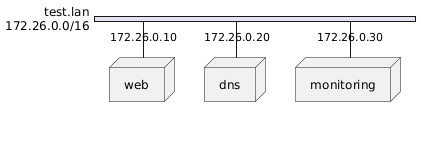
\includegraphics[width=\textwidth]{../graphics/nwdiag_test_env.png}
  \caption[Netwerkdiagram testomgeving in afbeeldingsformaat (PlantUML)]{Afbeeldingsformaat van het netwerkdiagram van de testomgeving, gegenereerd door PlantUML.}
  \label{fig:nwdiag_test_env.png}
\end{figure}

\subsubsection{Implementatiediagram}

Het \textbf{implementatiediagram} (\texttt{uml\_test\_env.puml}) toont de \emph{Ansible}-rollen die op elke host draaien en hun onderlinge verbindingen. Zo wordt in één oogopslag duidelijk welke hosts met elkaar communiceren en via welke rol. Dit diagram vormt samen met het netwerkdiagram de invoer voor de converter.

\subsection{Beperkingen}%

De volgende beperkingen gelden voor de testomgeving en bij uitbreiding voor de converter:

\begin{itemize}
\item De omgeving wordt lokaal opgezet via Vagrant en geconfigureerd via Ansible; de converter zal dus uitvoer genereren die op deze backends zijn afgestemd.
\item Enkel IPv4 wordt ondersteund bij het definiëren van netwerkadressen en host-IP's.
\item De control node (\texttt{172.26.255.253}) is aanwezig in \texttt{vagrant-hosts.yml} maar wordt niet gerepresenteerd in de netwerk- of implementatiediagrammen.
\item Routering en switching worden niet in rekening gebracht.
\end{itemize}